\section{Planning, affectation des taches}
\paragraph{} Nous nous sommes réunis pour discuter de la façon dont nous allions structurer notre travail, mais nous avons aussi mis en place une méthodologie afin d'avancer tous sur les même bases. Nous avons aussi mis en place un planning et un répartition du travail.
\subsection{Méthodologie}
\paragraph{} Concernant la voie à suivre pour notre travail de groupe ou individuel, nous nous sommes mis d'accord pour se concerter en début de chaque semaine, afin de faire le point sur l'avancement du travail jusqu'à la date de la réunion. Ce rendez-vous hebdomadaire a aussi pour but de fixer la répartition des taches pour la semaine qui suit, afin que chacun sache ce qu'il a à faire, et comment le faire au mieux.

\paragraph{} Le but de ces rencontres et aussi de pouvoir faire semaine par semaine un compte-rendu de l'avancement  au client (afin qu'il puisse suivre le développement du projet). Ce compte-rendu aura aussi pour objectif, du fait que notre client est aussi notre encadrant, de lui permettre de nous donner son avis sur notre organisation, étape par étape, ainsi que de voir avec lui au fur et à mesure que l'on avance, si nous répondons aux besoins, et de pouvoir lui poser des questions si nous rencontrons des difficultés.
\subsection{Répartition des taches} \paragraph{}
Nous avons constaté que deux grandes parties se distinguent dans ce TER. Comme expliqué dans l'analyse des besoins, il apparaît qu'il est facile de traiter chacune de leur coté, la partie concernant l'interface utilisateur, et la partie de gestion de la fenêtre 3D.

\paragraph{} 
Le groupe étant formé de quatre personnes, nous allons travailler par binôme, travaillant deux par deux sur chacune des parties du TER. Nous avons déjà travaillé avec OpenGL, et certain d'entre nous ont déjà travaillé avec RGL et Explorer3D. 

\paragraph{} Léo Rousseau qui a déja travaillé avec RGL, va de ce fait se concentrer sur la partie visualisation 3D du projet, ainsi que Julien Henry. Alexandre Masson ayant déja quelques connaissance sur le logiciel Explorer3D travaillera avec Nicolas Lacourte-Barbadaux sur la partie Rgtk et conception de l'interface utilisateur .

\newpage
\subsection{Planning Général}

\begin{center}
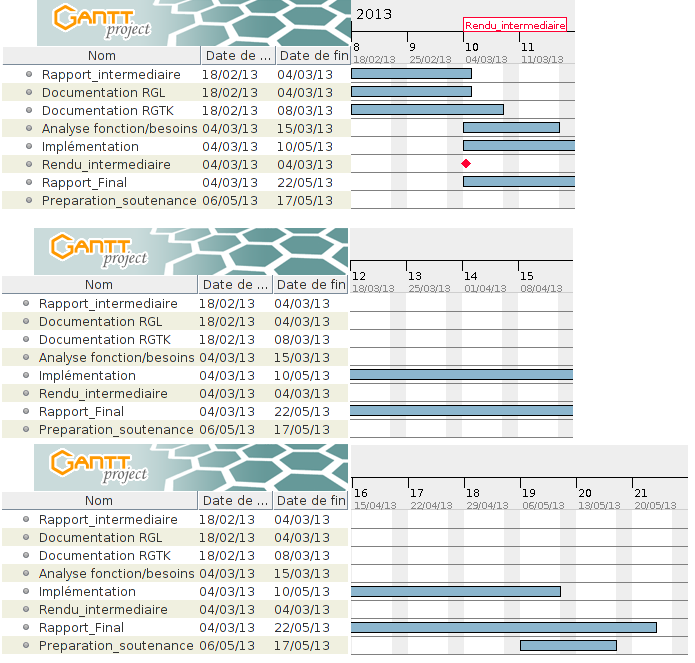
\includegraphics[scale=0.7]{diag_ter.png}
\end{center}
\newpage